%\newpage
\subsection{Cosmic Radiation}
\label{sec:Cosmic-Radiation-Results}
	
\subsubsection{Performance}

Overall the MiniPIX performed very well and exceeded all of the planned scientific goals, an example of one of the captured frames is given in Figure~\ref{fig:hits1}. Over the course of the flight our playoad collected a total of \num{7751} frames of correct and calibrated data while maintaining a temperature within the manufacturers specified operating range, as seen in Figure~\ref{fig:mp_pi_temps}. The data retrieved from the MiniPIX allowed us to create a vertical profile of atmospheric radiation and understand the dosage of cosmic radiation during the duration of our flight. This bodes very well for future flights as the MiniPIX combined with a RP3 is a very cheap and simple way to do fairly complex analysis of GCRs. Due to the monetary value of the MiniPIX it was also a concern that upon impact with the ground at the end of the flight it would be damaged beyond recovery, however, after testing post flight the device appears undamaged and operates normally. 

%\begin{wrapfigure}{r}{.30\textwidth}
\begin{figure}[H]
\begin{center}
%\vspace{-50pt}
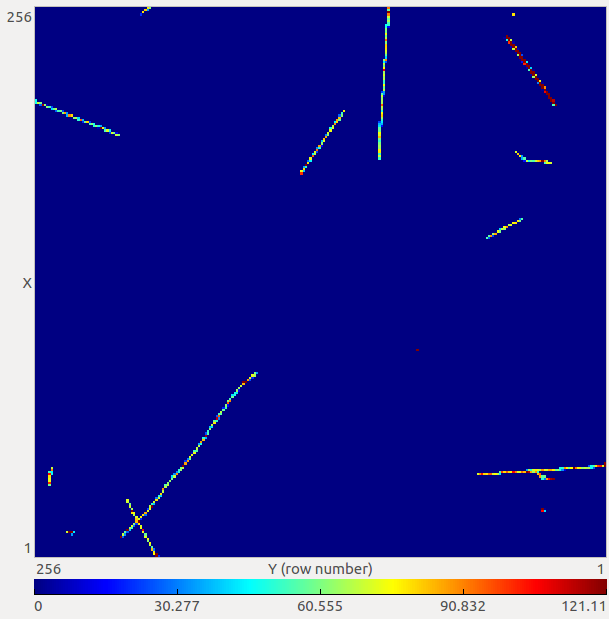
\includegraphics[width=.50\textwidth]{./Figures/flight_frame.png}
\caption{Frame collected during ascent, displayed using ADVACAM's PixetPro software.}
  %\vspace{-30pt}
\label{fig:hits1}
\end{center}
\end{figure}
%\end{wrapfigure} 

\begin{figure}[h!]
\begin{center}
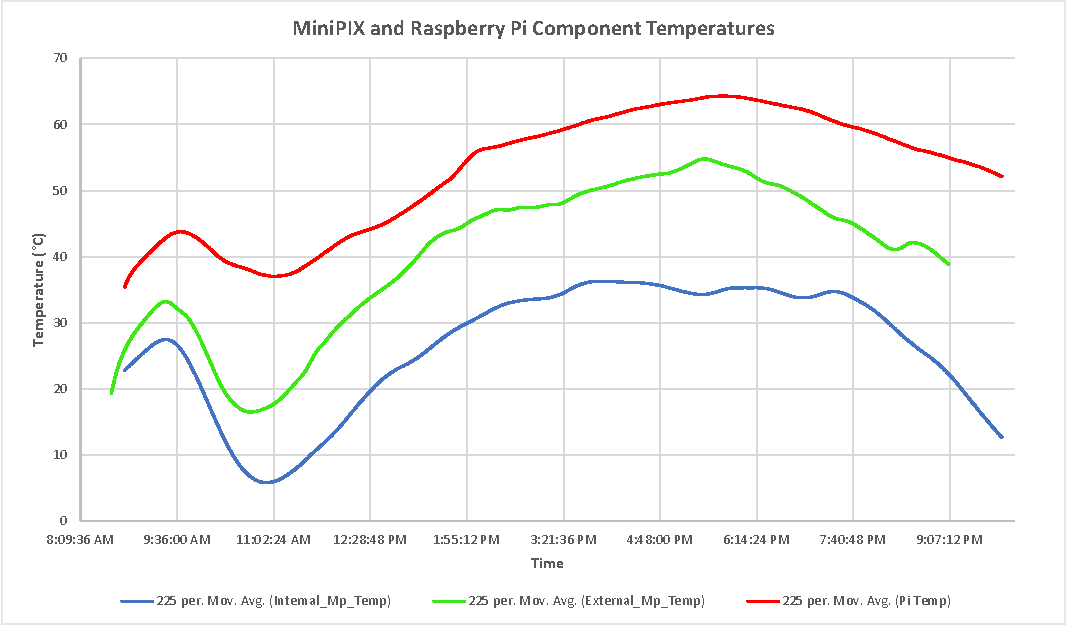
\includegraphics[width=0.95\textwidth]{./Figures/mp_pi_temps.pdf}
\caption{Temperatures of the MiniPIX and RP3 during the duration of the entire flight.}
\label{fig:mp_pi_temps}
\end{center}
\end{figure}
        
\subsubsection{Atmospheric Radiation Profile}

Assuming that each cluster in a frame corresponded to one hit on the detector we were able to plot the number of counts per frame over the duration of our flight. Count values for each frame were averaged over \SI{4000}{\feet} of altitude and the standard error was then calculated for each of those means. As shown in Figure~\ref{fig:hits2}, on the ascent up to approximately \SI{60000}{\feet} we see a direct correlation between altitude and rise in counts until reaching a peak. After which the hit rate decreases with increasing altitude until reaching float where it levels off at an average of about 8 hits per frame. This curve provides us a very clear picture of our payload passing through the Regener-Pfotzer Maximum~\cite{regener}. After sorting the detector hits into their appropriate morphological type and plotting them we were able to see that clusters identified as light tracks, straight tracks and small blobs showed a very prominent peak, this is shown in Figure~\ref{fig:clustersplot}. This is logical as these tracks morphological classifications generally correspond to the types of particles that we would expect for secondary cosmic ray interactions which should reach a maximum in this layer of the atmosphere. That is, they are representative of muons, fast protons, pions, electrons and low energy short range particle interactions~\cite{stuartthesis}.

\begin{figure}[h!]
\begin{center}
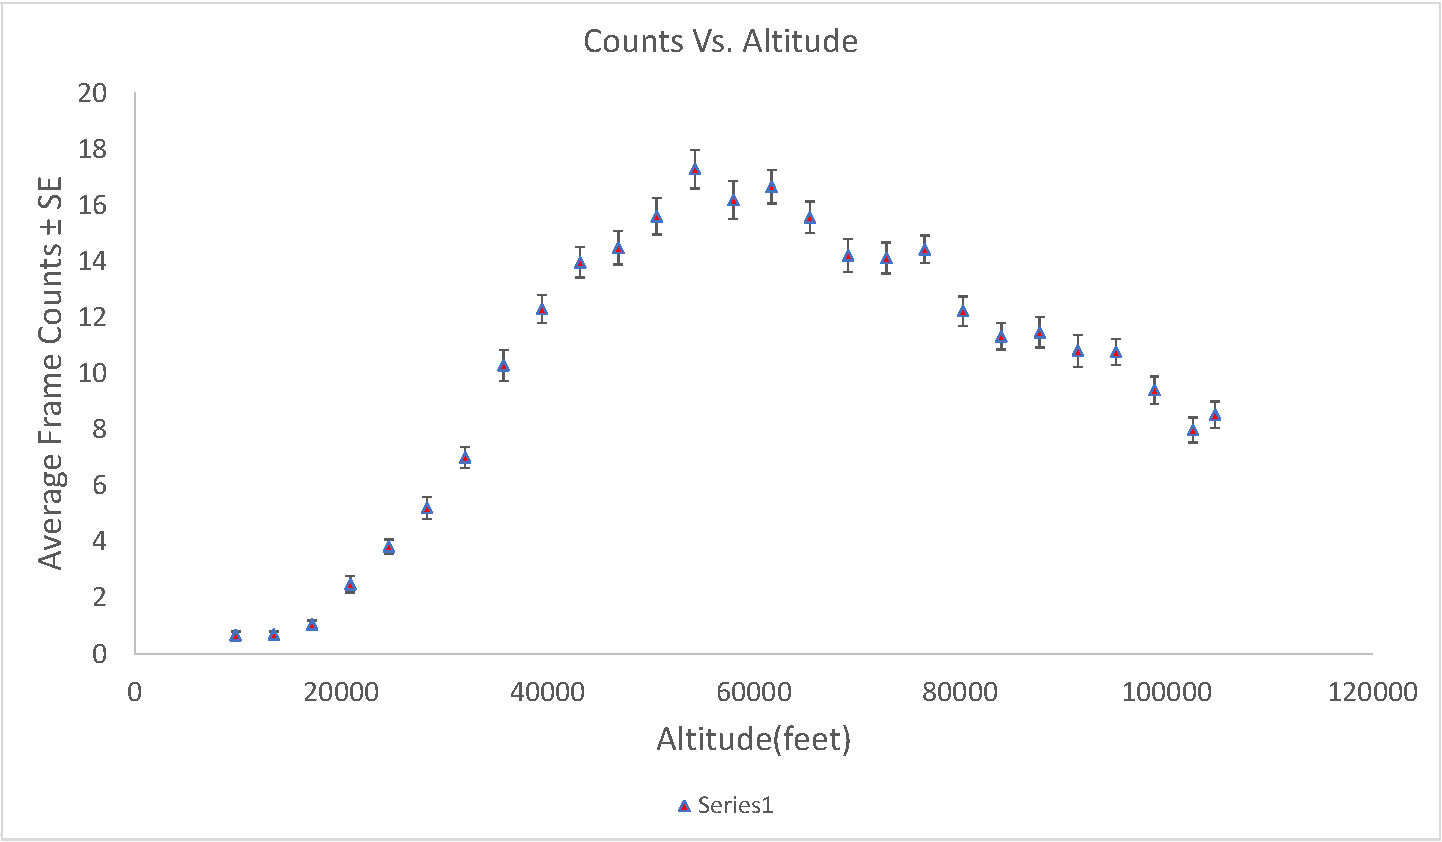
\includegraphics[width=.9\textwidth]{./Figures/countstderr.pdf}
\caption{Plot of total detector hits per frame averaged over 4000 ft high bins}
\label{fig:hits2}
\end{center}
\end{figure}

\begin{figure}[h!]
\begin{center}
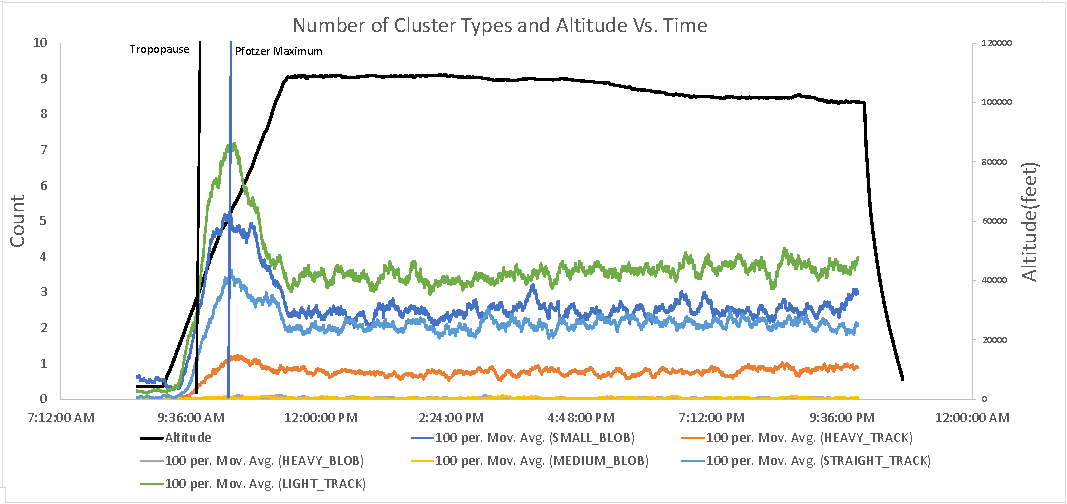
\includegraphics[width=0.8\textwidth]{./Figures/typesandaltitudevtime.pdf}
\caption{Plot of counts of hits sorted by morphological type and altitude vs time over the duration of our flight.}
\label{fig:clustersplot}
\end{center}
\end{figure}


We were also able to calculate the absorbed dose for each frame of data. To determine the absorbed dose we took the total amount of energy deposited on a frame and divided it by the mass of our detector. Let $E_{f}$ be the total amount of energy in joules deposited on one frame and $\rho$ be the density of silicon. The MiniPIX detector is \SI{500}{\micro\meter} thick and has $256^2$ pixels, each pixel has a pitch of \SI{55}{\micro\meter}. The calculations for the mass of our detector and absorbed dose in silicon $D_{Si}$ are shown in Eq.~(\ref{eq:detmass}) and Eq.~(\ref{eq:detdose}), respectively.

	\begin{equation}
	M_{d} = 256^2 \cdot \SI{55}{\micro\meter}^2 \cdot \SI{500}{\micro\meter} \cdot \rho
      	\label{eq:detmass}
	\end{equation}
	\begin{equation}
	D_{Si} = \frac{E_{f}}{M_{d}}
	\label{eq:detdose}
	\end{equation}

The dose rate per minute was calculated by taking the absorbed dose rate divided by the shutter time and multiplying it by \num{60}, the values for each frame were then averaged over each increase of \SI{4000}{\feet} in altitude. The plot of dose rate over altitude, shown in Figure~\ref{fig:doserate}, was generated using the same method as above for the counts plot and shows a very similar shape to that of the counts plot however its peak seems to be slightly higher at around \SI{65000}{\feet} and it does not decrease as rapidly after reaching its maximum. As you can see from the graph the error bars increase in range as altitude increases, this can be explained by the data being skewed by a small number of very high energy hits on the detector or nuclear interactions. The vertical profile of dose rate is variable based on latitude and other factors but is generally lower near the equator and higher towards the poles. Our data seems to match very closely with data collected at similar latitudes.


\begin{figure}[h!]
\begin{center}

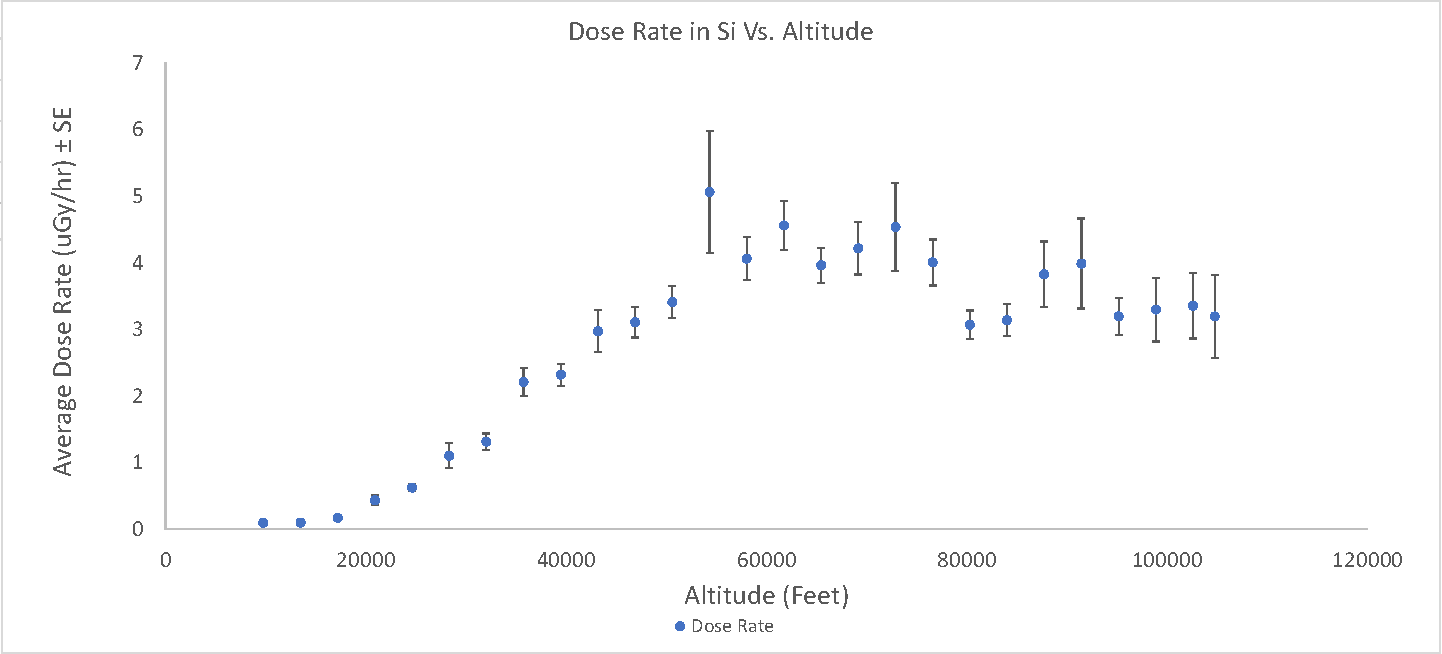
\includegraphics[width=0.8\textwidth]{./Figures/dosestderr.pdf}
\caption{Dose rate during flight.  The dose rate peaked at about \SI{4.2}{\micro\gray\per\hour} and then leveled off at about \SI{3}{\micro\gray\per\hour} at float. This is consistent with other data collected on balloon flights at similar latitudes such as that of the Intercontinental Space Weather Balloon Network 2016--2017 campaign's flight in california~\cite{spaceballoonnetwork}, see Appendix~\ref{sec:appendixa}.}
\label{fig:doserate}
\end{center}
\end{figure}


\subsubsection{Particle Interactions}

%\begin{wrapfigure}{R}{.3\textwidth}
\begin{figure}[H]
\begin{center}
%\vspace{-25pt}
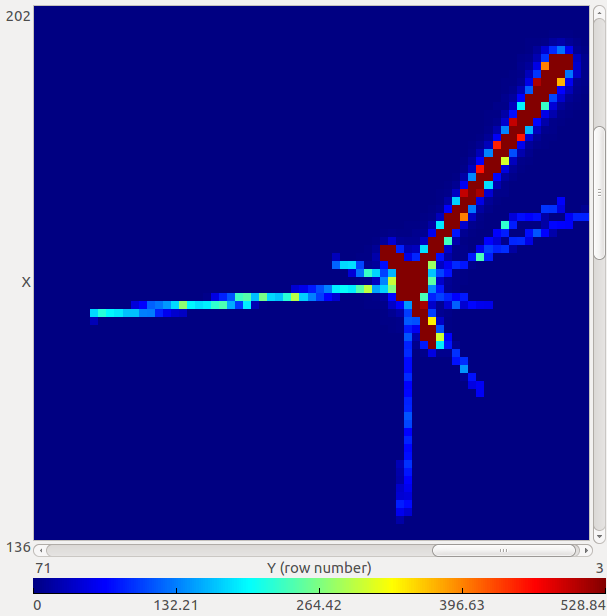
\includegraphics[width=.5\textwidth]{./Figures/nuclear_interaction.png}
\caption{Example of a nuclear interaction in the MiniPIX detector recorded during flight.}
%  \vspace{-90pt}
\label{fig:hits3}

\end{center}
%\end{wrapfigure} 
\end{figure}

During the course of the flight we received many tracks on the detector that did not fit nicely into any of the morphological categories defined by the sorting algorithm. These tracks are likely from interactions between GCRs and atoms in the surrounding material of the MiniPIX and looked like the event shown in Figure~\ref{fig:hits3}. The proportion of these tracks compared to the overall population of tracks recorded is fairly small so its unlikely that it had any significant affect on the overall morphological analysis. These tracks are interesting nonetheless, even if their analysis is beyond the scope of this report. Hopefully further analysis of these interactions can be performed in future publications.

\subsubsection{UV Radiation}
\label{sec:UV-Radiation-Results}

%Give intro to the valuable information we learned from the data and overview of the graphs to be discussed. 
The UV irradiance measured as a function of the payload's altitude is shown for each of the three UV sensors in Figure~\ref{fig:uv_altitude}, with each graph scaled the same to allow for easy comparison. The peaks for each UV sensor are as follows: \SI{47.96}{\watt\per\meter\squared}, \SI{31.98}{\watt\per\meter\squared}, and \SI{25.16}{\watt\per\meter\squared} for UV$_0$, UV$_1$, and UV$_2$ respectively. From these graphs, it is obvious that the peak UV readings occur during the float altitude. This implies that the peak UV readings are essentially, for all intents and purposes of our experiment, independent of altitude.

\begin{figure}[]
\begin{center}
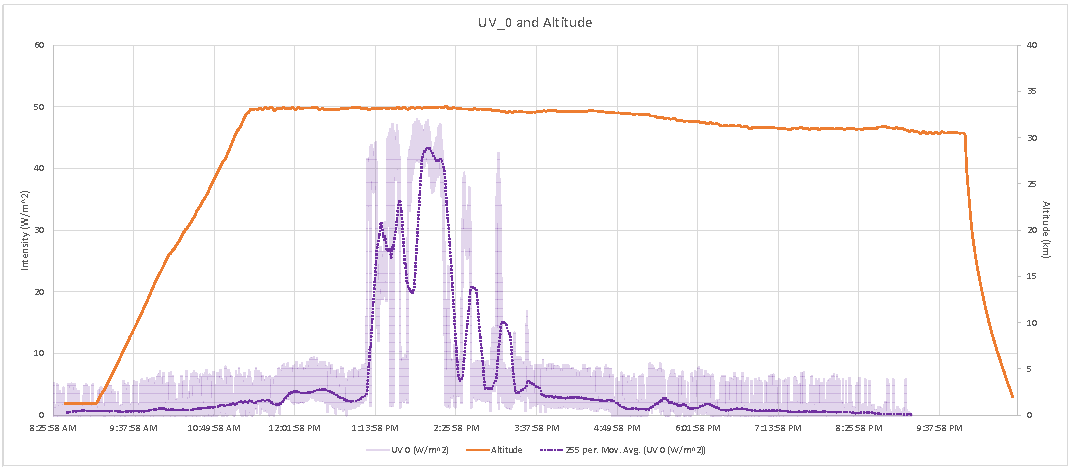
\includegraphics[width=0.8\textwidth]{./Figures/uv_0_graph.pdf}
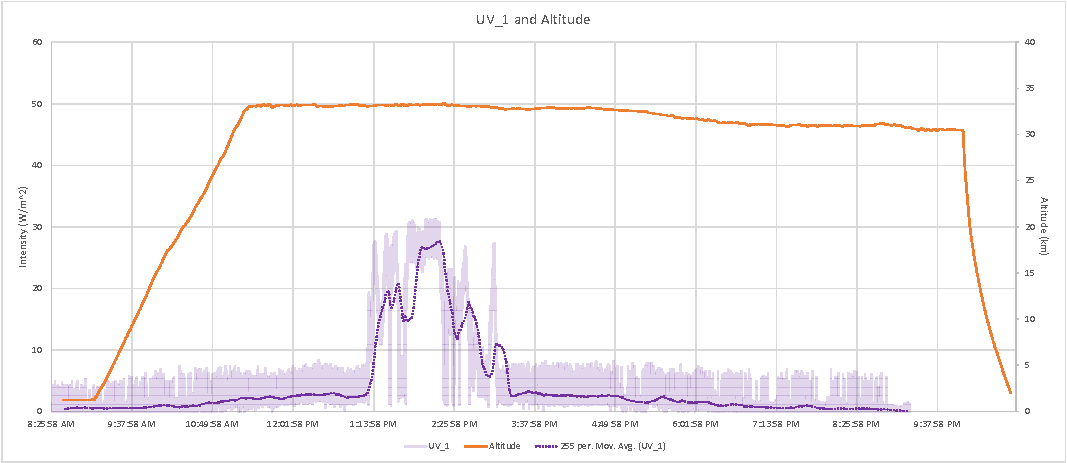
\includegraphics[width=0.8\textwidth]{./Figures/uv_1_graph.pdf}
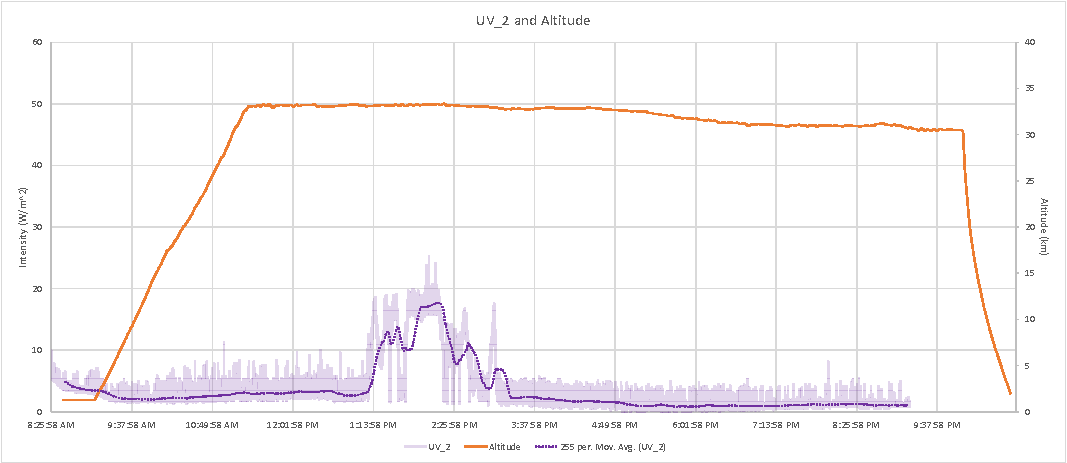
\includegraphics[width=0.8\textwidth]{./Figures/uv_2_graph.pdf}
\caption{UV sensor readings with altitude.  Top, middle and bottom show the measurement from the UV$_0$, UV$_1$ and UV$_2$ photodiodes, respectively.}
\label{fig:uv_altitude} 
\end{center}
\end{figure}



	
	
%	\begin{figure}[!hbp]
%	\begin{center}
%	\begin{minipage}[b]{0.49\textwidth}
%	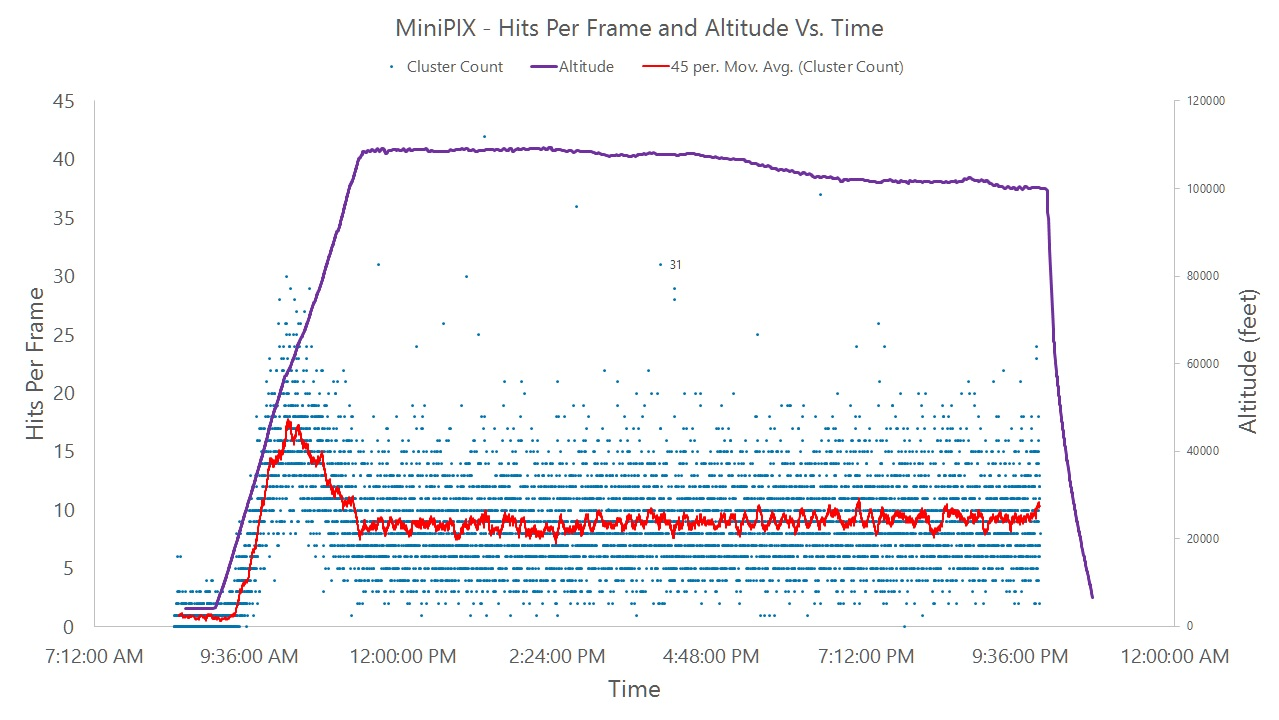
\includegraphics[width=\textwidth]{./Figures/hitsvaltitudevtime.jpg}
%	\caption{Plot of hits and altitude over the duration of our flight.}
%	\label{fig:uv_0_altitude} 
%	\end{minipage}
%	%\end{center}
%	%\end{figure}
%	\hfill
%	%\begin{figure}[!htb]
%	%\begin{center}
%	\begin{minipage}[b]{0.49\textwidth}
%	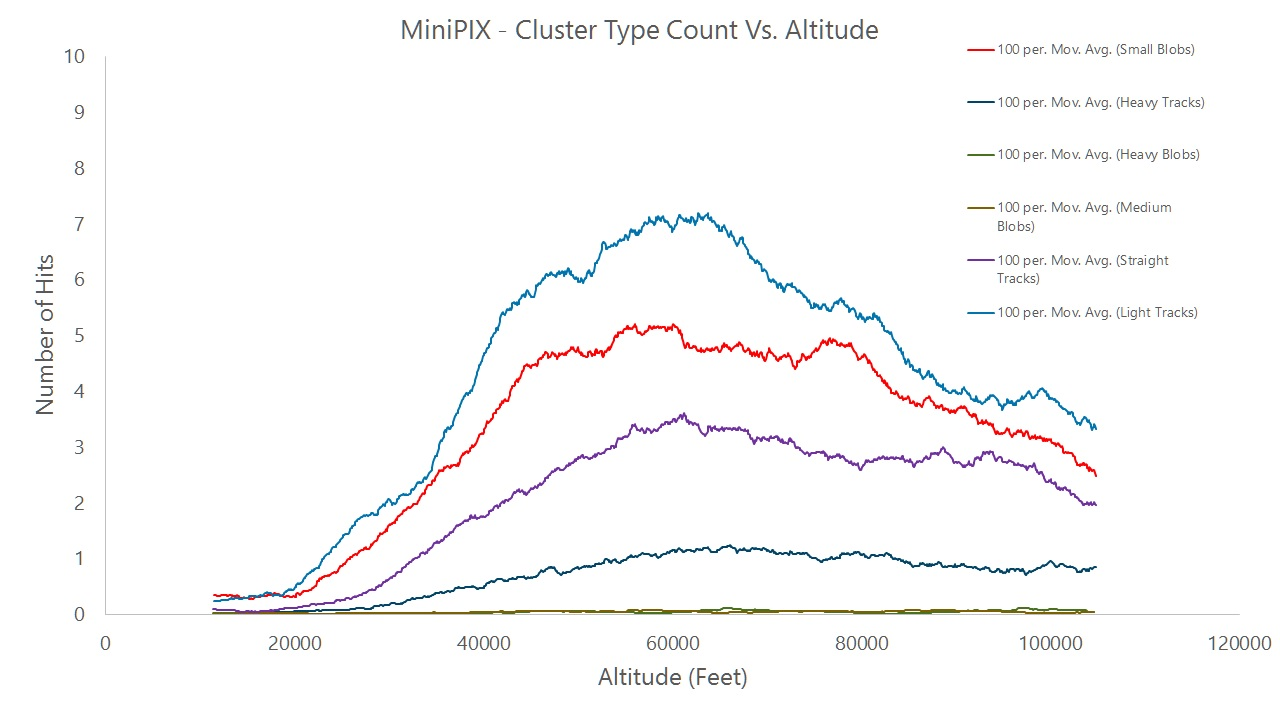
\includegraphics[width=\textwidth]{./Figures/clustervaltitude_big.jpg}
%	\caption{Plot of hits and altitude over the duration of our flight.}
%	\label{fig:uv_1_altitude} 
%	\end{minipage}
%	\end{center}
%	\end{figure}
%	
